\documentclass[12pt]{article}
\usepackage[utf8]{inputenc}
\usepackage[T1]{fontenc}
\usepackage{graphicx} % Para insertar imágenes
\usepackage{amsmath} % Matemáticas avanzadas
\usepackage{hyperref} % Hipervínculos
\usepackage{setspace} % Control de interlineado
\usepackage{xcolor} % Colores
\usepackage{enumitem} % Listas personalizadas
\usepackage{booktabs} % Tablas profesionales
\usepackage{geometry} % Márgenes personalizados
\usepackage{float} % Posicionamiento de figuras y tablas
\usepackage{multirow} % Celdas combinadas en tablas
\usepackage{tcolorbox}
\usepackage{listings}
\usepackage{float}      % Control de posicionamiento
\usepackage{placeins} 


% Configuración de márgenes
\geometry{a4paper, margin=1in}

\lstdefinestyle{python}{
	language=Python,
	backgroundcolor=\color{white},
	basicstyle=\footnotesize\ttfamily,
	keywordstyle=\color{blue},
	commentstyle=\color{green!50!black},
	stringstyle=\color{red},
	numbers=left,
	numberstyle=\tiny\color{gray},
	stepnumber=1,
	numbersep=5pt,
	frame=single,
	breaklines=true,
	showspaces=false,
	showstringspaces=false,
}

% Configuración de hipervínculos
\hypersetup{
	colorlinks=true,
	linkcolor=blue,
	filecolor=magenta,      
	urlcolor=cyan,
}

% Estilo de listas
\setlist[itemize]{noitemsep, topsep=0pt} % Reduce el espacio en listas

% Colores para código
\definecolor{codegreen}{rgb}{0,0.6,0}
\definecolor{codegray}{rgb}{0.5,0.5,0.5}
\definecolor{codepurple}{rgb}{0.58,0,0.82}
\definecolor{backcolour}{rgb}{0.95,0.95,0.92}
	
\begin{document}
	
	%%%%%%%%%%%%%%%%%%%%%%%%%%%%%%%%%%%%%%%%%%%%%%%%%%%%%%%%%%%%%%%%%%%%%%%%
    \chapter{Optimización Multiobjetivo para la Toma de Decisiones en Políticas Públicas}
    \textbf{Autor}: \large{Eder Luna O.}
    \label{chap:11}
	
	\subsection*{Introducción}
	
	La optimización multiobjetivo (MO) y la toma de decisiones de múltiples criterios (MCDM) permiten evaluar soluciones que equilibran objetivos en conflicto, siendo fundamentales en la asignación de recursos, el diseño de políticas públicas y la evaluación de programas sociales \cite{Sengupta2016}. En este contexto, herramientas como pymoo han surgido para facilitar la optimización de múltiples objetivos, ofreciendo visualización de soluciones, personalización de algoritmos y métodos de toma de decisiones con múltiples criterios \cite{Blank2020}.  
	
	En políticas públicas, la optimización multiobjetivo permite modelar y visualizar compensaciones entre eficiencia y equidad, facilitando decisiones más informadas y participativas \cite{Papalexopoulos2022}. Su aplicación en sectores como educación y salud mejora la eficiencia y asegura que las decisiones sean inclusivas y justas, fortaleciendo el impacto de las políticas.
	
	\subsection{Optimalidad de Pareto y Compensaciones Multiobjetivo}
	
	La \textbf{Optimalidad de Pareto} es un principio fundamental en la optimización multiobjetivo, donde una solución se considera óptima si no es posible mejorar un objetivo sin afectar negativamente al menos otro. Esto permite analizar compensaciones entre objetivos en problemas con múltiples criterios en conflicto.  
	
	En la gestión ambiental, la \textit{optimización de Pareto} se ha aplicado para equilibrar intereses divergentes. Kennedy et al. \cite{Kennedy2008} destacan que este enfoque permite a los responsables de decisiones visualizar las compensaciones entre objetivos sin necesidad de ponderaciones previas, facilitando una toma de decisiones más informada.  
	
	Uno de los métodos más utilizados es el algoritmo evolutivo multiobjetivo \textbf{NSGA-II}, que ha demostrado ser eficaz en diversas aplicaciones \cite{Confesor2007}. Por ejemplo, en la calibración automática del modelo hidrológico SWAT, se optimizaron múltiples parámetros simultáneamente, mejorando la simulación del caudal en cuencas hidrográficas. Este enfoque también es útil en la formulación de políticas, permitiendo equilibrar objetivos como el desarrollo económico y la calidad ambiental.  
	
	Un caso práctico de aplicación es el diseño de estrategias de gestión forestal, donde se busca minimizar el impacto del fuego, proteger hábitats de especies en peligro y preservar reservas forestales. La frontera de Pareto proporciona un conjunto de soluciones óptimas, facilitando decisiones más equilibradas y consensuadas.  
	
	
	
	\section*{Ejemplo:}
	Supongamos que tenemos un río del cual se extrae agua para dos propósitos principales:
	\textbf{Suministro de agua para riego agrícola} (objetivo 1: maximizar).
	\textbf{Mantener un caudal ecológico mínimo} para preservar la salud del ecosistema acuático (objetivo 2: minimizar la desviación del caudal ecológico).
	
	Estos dos objetivos están en conflicto porque, si se extrae más agua para la agricultura, el caudal ecológico se reduce, lo que puede dañar el ecosistema. Por otro lado, si se prioriza el caudal ecológico, se reduce el agua disponible para la agricultura.
	
	\section*{Enfoque de Optimalidad de Pareto}
	Para resolver este problema, aplicamos un enfoque de optimización multiobjetivo. El objetivo es encontrar un conjunto de soluciones que representen las compensaciones entre los dos objetivos. Estas soluciones forman la \textbf{frontera de Pareto}.
	
	\subsection*{Pasos del ejemplo}
	
	\subsubsection*{Paso 1: Definir las variables de decisión}  
	\begin{itemize}
		\item \( x \): Cantidad de agua extraída para riego agrícola (en millones de metros cúbicos por año).
	\end{itemize}
	
	\subsubsection*{Paso 2: Definir los objetivos}  
	\begin{itemize}
		\item \textbf{Objetivo 1 (maximizar):} Suministro de agua para riego agrícola.
		\[
		f_1(x) = x
		\]
		\item \textbf{Objetivo 2 (minimizar):} Desviación del caudal ecológico mínimo.
		\[
		f_2(x) = \text{Caudal ecológico mínimo} - (\text{Caudal total} - x)
		\]
		Supongamos que el caudal total del río es de 100 millones de m³/año y el caudal ecológico mínimo requerido es de 40 millones de m³/año. Entonces:
		\[
		f_2(x) = 40 - (100 - x) = x - 60
		\]
	\end{itemize}
	
	\subsubsection*{Paso 3: Definir las restricciones}  
	\begin{itemize}
		\item La cantidad de agua extraída no puede superar el caudal total:
		\[
		x \leq 100
		\]
		\item El caudal ecológico no puede ser menor que el mínimo requerido:
		\[
		100 - x \geq 40 \implies x \leq 60
		\]
	\end{itemize}
	
	
	\subsubsection*{Paso 4: Generar soluciones posibles:}
	\begin{itemize}
		\item Variamos \( x \) desde 0 hasta 60 (el límite superior permitido por la restricción del caudal ecológico).
		\item Para cada valor de \( x \), calculamos \( f_1(x) \) y \( f_2(x) \).
	\end{itemize}
	
	\subsubsection*{Paso 5: Resultados:}
	\begin{itemize}
		\item Si \( x = 0 \): No se extrae agua para agricultura (\( f_1 = 0 \)), pero el caudal ecológico es máximo (\( f_2 = -60 \)).
		\item Si \( x = 60 \): Se extrae la máxima cantidad permitida para agricultura (\( f_1 = 60 \)), pero el caudal ecológico es igual al mínimo requerido (\( f_2 = 0 \)).
	\end{itemize}
	
	\begin{table}[h!]
		\centering
		\begin{tabular}{ccc}
			\toprule
			\( x \) (millones de m³/año) & \( f_1(x) \) (agricultura) & \( f_2(x) \) (desviación ecológica) \\
			\midrule
			0                             & 0                          & -60                                 \\
			20                            & 20                         & -40                                 \\
			40                            & 40                         & -20                                 \\
			60                            & 60                         & 0                                   \\
			\bottomrule
		\end{tabular}
		\caption{Resultados de las soluciones posibles.}
	\end{table}
	
	\textbf{Frontera de Pareto:}
	\begin{itemize}
		\item Las soluciones óptimas de Pareto son aquellas en las que no se puede mejorar un objetivo sin empeorar el otro. En este caso, todas las soluciones con \( x \) entre 0 y 60 son óptimas de Pareto.
		\item Por ejemplo:
		\begin{itemize}
			\item Si elegimos \( x = 20 \), podemos aumentar \( x \) a 40 para mejorar la agricultura, pero esto empeora la desviación ecológica.
			\item Si elegimos \( x = 40 \), podemos reducir \( x \) a 20 para mejorar el caudal ecológico, pero esto reduce el suministro agrícola.
		\end{itemize}
	\end{itemize}
\end{enumerate}

\subsection*{Visualización de la frontera de Pareto}
Podemos graficar los dos objetivos para visualizar la frontera de Pareto:

\begin{itemize}
	\item Eje X: \( f_1(x) \) (Suministro agrícola).
	\item Eje Y: \( f_2(x) \) (Desviación ecológica).
\end{itemize}

La curva que conecta los puntos \((0, -60)\), \((20, -40)\), \((40, -20)\) y \((60, 0)\) representa la frontera de Pareto. Cualquier punto fuera de esta curva es dominado por al menos un punto en la curva.

\begin{figure}[h]
	\centering
	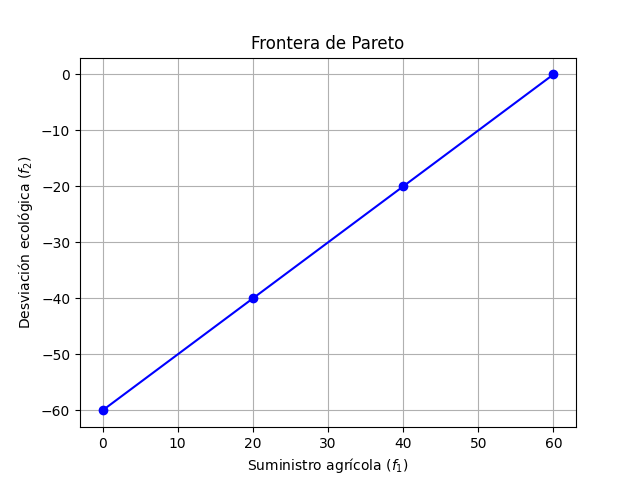
\includegraphics[width=0.9\linewidth]{Figure_pareto.png}
	\caption{Frontera de Pareto}
	\label{Pareto}
\end{figure}

\clearpage  % Asegura que la imagen esté separada del siguiente contenido

\subsection*{Código}
\begin{lstlisting}[style=python]
	import matplotlib.pyplot as plt
	
	# Datos
	f1 = [0, 20, 40, 60]  # Suministro agrícola
	f2 = [-60, -40, -20, 0]  # Desviación ecológica
	
	# Gráfica
	plt.plot(f1, f2, marker='o', linestyle='-', color='b')
	plt.xlabel('Suministro agrícola ($f_1$)')
	plt.ylabel('Desviación ecológica ($f_2$)')
	plt.title('Frontera de Pareto')
	plt.grid(True)
	plt.savefig('pareto_front.png')  # Guardar la imagen
	plt.show()
\end{lstlisting}

Este ejemplo muestra cómo la \textbf{Optimalidad de Pareto} permite a los responsables de la toma de decisiones visualizar las compensaciones entre dos objetivos en conflicto. En este caso, se puede elegir entre:
\begin{itemize}
	\item Priorizar la agricultura (extraer más agua).
	\item Priorizar el ecosistema (extraer menos agua).
\end{itemize}

La frontera de Pareto proporciona un conjunto de soluciones que equilibran ambos objetivos, ayudando a tomar decisiones informadas y consensuadas. Este enfoque es especialmente útil en problemas ambientales, donde es común enfrentar múltiples objetivos en conflicto.

\subsection{Compensaciones Multiobjetivo}

Las \textit{compensaciones multiobjetivo} son un concepto clave en la toma de decisiones cuando se enfrentan múltiples objetivos que pueden entrar en conflicto. Estas compensaciones surgen cuando mejorar un objetivo implica necesariamente perjudicar otro, lo que obliga a los tomadores de decisiones a priorizar entre ellos. Este tipo de análisis es fundamental en áreas como la gestión ambiental, las políticas públicas y la asignación de recursos, donde se deben equilibrar intereses diversos y frecuentemente contrapuestos.

En el contexto de la gestión de tierras con múltiples objetivos, \cite{Bradford2012} destacan que, a medida que los objetivos de gestión y conservación de los recursos naturales se han diversificado, se vuelve esencial evaluar las consecuencias de diferentes opciones de manejo. Los autores proponen un enfoque que permite cuantificar los efectos de dichas opciones en términos de beneficios y compensaciones entre objetivos. Como mencionan, “los beneficios positivos resultantes de algunas opciones de gestión a menudo se asocian con grandes compensaciones entre objetivos individuales” \cite{Bradford2012}. Este análisis cuantitativo ayuda a los gestores y responsables de políticas a comprender los compromisos necesarios y a tomar decisiones informadas que equilibren intereses diversos.

Por otro lado, \cite{Couckuyt2014} argumentan que "un enfoque mejor es usar métodos de optimización multiobjetivo para identificar directamente un conjunto de soluciones óptimas de Pareto, que el diseñador puede usar para tomar decisiones de diseño más eficientes."

Un caso práctico de este tipo de análisis se encuentra en la gestión forestal a largo plazo, donde se han identificado compromisos significativos entre el ciclo del carbono y la complejidad ecológica. Este tipo de compensaciones es común en sistemas ambientales, donde los beneficios para un aspecto del ecosistema (como el secuestro de carbono) pueden requerir sacrificios en otros (como la biodiversidad).


\section*{}
En problemas de optimización multiobjetivo, las \textbf{compensaciones} se refieren a la necesidad de sacrificar el desempeño de un objetivo para mejorar el de otro. Estas compensaciones son inevitables cuando los objetivos están en conflicto, como en el caso de maximizar el suministro de agua para la agricultura y minimizar el impacto ambiental en un ecosistema acuático.

\subsection*{Compensaciones Multiobjetivo}

La optimización multiobjetivo busca minimizar o maximizar múltiples funciones objetivo simultáneamente. En este ejemplo, utilizamos el algoritmo NSGA-II (Non-dominated Sorting Genetic Algorithm II) para resolver un problema de optimización biobjetivo.

\subsection*{Definición del Problema}

Se consideran las siguientes funciones objetivo a minimizar:

\begin{align}
	f_1(x, y) &= x^2 + y^2 \\
	f_2(x, y) &= (x - 1)^2 + (y + 1)^2
\end{align}

donde $x$ e $y$ son las variables de decisión restringidas por:

\begin{align}
	-2 \leq x \leq 2, \quad -2 \leq y \leq 2.
\end{align}

\subsection*{Implementación en Python}

El código en Python para resolver este problema utilizando NSGA-II es:

\subsection*{Código}
\begin{lstlisting}[style=python]
	import numpy as np
	from pymoo.algorithms.moo.nsga2 import NSGA2
	from pymoo.optimize import minimize
	from pymoo.core.problem import Problem
	from pymoo.factory import get_sampling, get_crossover, get_mutation, get_termination
	import matplotlib.pyplot as plt
	
	class MyProblem(Problem):
	def __init__(self):
	super().__init__(n_var=2, n_obj=2, n_constr=0, xl=np.array([-2, -2]), xu=np.array([2, 2]))
	
	def _evaluate(self, X, out, *args, **kwargs):
	f1 = X[:,0]**2 + X[:,1]**2
	f2 = (X[:,0] - 1)**2 + (X[:,1] + 1)**2
	out["F"] = np.column_stack([f1, f2])
	
	problem = MyProblem()
	
	algorithm = NSGA2(
	pop_size=100,
	sampling=get_sampling("real_random"),
	crossover=get_crossover("real_sbx", prob=0.9, eta=15),
	mutation=get_mutation("real_pm", eta=20),
	eliminate_duplicates=True
	)
	
	res = minimize(problem, algorithm, termination=get_termination("n_gen", 100), seed=1, verbose=True)
	
	F = res.F
	plt.scatter(F[:,0], F[:,1], c='red')
	plt.xlabel("f1(x,y)")
	plt.ylabel("f2(x,y)")
	plt.title("Frente de Pareto")
	plt.show()
	
	def print_solutions():
	print("x\ty\tf1(x,y)\tf2(x,y)")
	for i in range(len(res.X)):
	print(f"{res.X[i,0]:.4f}\t{res.X[i,1]:.4f}\t{res.F[i,0]:.4f}\t{res.F[i,1]:.4f}")
	print_solutions()
\end{lstlisting}

\subsection*{Interpretación de Resultados}

Cada solución obtenida representa un punto en el \textbf{frente de Pareto}, donde ninguna solución es estrictamente mejor que otra en ambos objetivos simultáneamente.

Salida:
\begin{center}
	\ttfamily
	x       y       f1(x,y)  f2(x,y) \\
	-------------------------------- \\
	1.0016  -0.9954  1.9940   0.0000 \\
	0.0049   0.0016  0.0000   1.9935 \\
	...
\end{center}

\subsection*{Análisis de las Soluciones}

Cada fila representa una solución óptima:
- $x$ e $y$ son las variables de decisión.
- $f_1(x,y)$ y $f_2(x,y)$ son los valores de las funciones objetivo.

En el caso de la solución:
\begin{center}
	(1.0016, -0.9954) \Rightarrow f_1(1.0016, -0.9954) = 1.9940, \quad f_2(1.0016, -0.9954) = 0.0000
\end{center}

Esta solución minimiza $f_2(x,y)$, pero con un costo en $f_1(x,y)$. Si la prioridad fuera minimizar $f_1(x,y)$, la mejor opción sería:
\begin{center}
	(0.0049, 0.0016) \Rightarrow f_1(0.0049, 0.0016) = 0.0000, \quad f_2(0.0049, 0.0016) = 1.9935
\end{center}

\subsection*{Gráfico del Frente de Pareto}

El gráfico generado muestra los puntos óptimos obtenidos:

\begin{figure}[H]
	\centering
	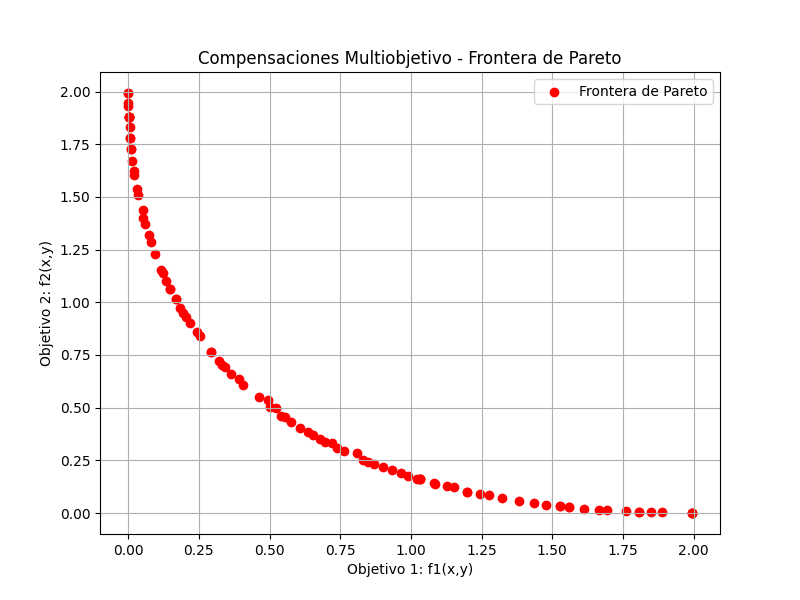
\includegraphics[width=0.9\linewidth]{Figure_2.png}
	\caption{Compensación Multiobjetivo}
	\label{fig:frente-pareto}
\end{figure}

Los puntos más a la izquierda minimizan $f_1(x,y)$ y los más abajo minimizan $f_2(x,y)$. La elección de la mejor solución depende de la prioridad entre los objetivos.El algoritmo NSGA-II proporciona un conjunto de soluciones óptimas para problemas multiobjetivo. La interpretación de estas soluciones permite tomar decisiones informadas en función de las preferencias del problema.


\subsection{Métodos de Suma Ponderada y $\varepsilon$-Restricción}

\subsubsection{Modelo de Suma Ponderada (WSM)}

El Modelo de Suma Ponderada (\textit{Weighted Sum Model, WSM}) es una técnica comúnmente utilizada en la toma de decisiones multicriterio (\textit{MCDM, por sus siglas en inglés}) que permite combinar varios criterios de decisión en un único valor agregado. Este modelo es particularmente útil cuando los tomadores de decisiones se enfrentan a múltiples objetivos que pueden ser conflictivos entre sí, y necesitan una forma de evaluar alternativas que considere la importancia relativa de cada objetivo.

Como se menciona en \cite{Marler2010}, "Minimizar una suma ponderada constituye un método independiente y un componente de otros métodos. En consecuencia, conocer las características del método de la suma ponderada tiene implicaciones de largo alcance."

\paragraph{Definición:}
El WSM se basa en la agregación de criterios utilizando ponderaciones asignadas a cada criterio según su importancia relativa. En este modelo, cada alternativa se evalúa en función de todos los criterios, y cada puntuación de criterio se multiplica por una ponderación predefinida. Luego, los resultados ponderados se suman para obtener una puntuación final para cada alternativa.

La fórmula general del modelo de suma ponderada es la siguiente:

\[
S_j = \sum_{i=1}^n w_i x_{ij}
\]

donde:
\begin{itemize}
	\item $S_j$ es la puntuación global de la alternativa $j$,
	\item $w_i$ es la ponderación del criterio $i$,
	\item $x_{ij}$ es la puntuación de la alternativa $j$ para el criterio $i$,
	\item $n$ es el número total de criterios.
\end{itemize}

\paragraph{Aplicación en la toma de decisiones:}
El WSM es especialmente útil en situaciones donde:
\begin{enumerate}
	\item Múltiples criterios deben ser considerados al evaluar alternativas.
	\item Los criterios pueden ser conflictivos entre sí (por ejemplo, costo versus calidad).
	\item Se puede asignar una ponderación para reflejar la importancia relativa de cada criterio.
\end{enumerate}

Este modelo se utiliza en diversos campos, como la gestión de proyectos, la planificación urbana, la evaluación de inversiones y la gestión ambiental, entre otros.

\paragraph{Ejemplo de Aplicación:}
Un ejemplo claro de aplicación del Modelo de Suma Ponderada es el estudio realizado en Popayán, Colombia, para la mejora de las calles de la ciudad. En este caso, se utilizó el WSM para evaluar qué tan cerca estaban los segmentos de calles de cumplir con los estándares de calidad y funcionalidad. El estudio consideró criterios como seguridad, sostenibilidad y accesibilidad, a los cuales se les asignó una ponderación específica según su importancia. Posteriormente, se evaluaron las alternativas de mejora, sumando las puntuaciones ponderadas para determinar las mejores opciones  \cite{Alban2023}.

\paragraph{Ventajas del Modelo de Suma Ponderada:}
\begin{itemize}
	\item \textbf{Simplicidad y Facilidad de Uso:} Es fácil de aplicar y entender, lo que lo hace accesible incluso para tomadores de decisiones sin formación técnica avanzada.
	\item \textbf{Flexibilidad:} Puede ser utilizado con cualquier número de criterios y en una amplia variedad de contextos.
	\item \textbf{Transparencia:} Las decisiones tomadas utilizando WSM son fácilmente explicables, ya que se basan en una suma de componentes con lógica clara.
	\item \textbf{Facilidad para Incorporar Juicios Expertos:} Las ponderaciones pueden ser ajustadas por expertos para reflejar prioridades o valores específicos.
\end{itemize}

\paragraph{Desventajas:}
\begin{itemize}
	\item \textbf{Subjetividad en la Asignación de Ponderaciones:} Las ponderaciones pueden ser arbitrarias o subjetivas, lo que puede llevar a decisiones sesgadas si no se manejan cuidadosamente.
	\item \textbf{No Captura la Relación entre Criterios:} El WSM asume que los criterios son independientes entre sí, lo que no siempre es cierto.
	\item \textbf{No es Adecuado para Problemas No Lineales:} En algunos casos, la relación entre los criterios y las alternativas no es lineal, lo que reduce la efectividad del modelo.
\end{itemize}

\subsubsection*{Suma Ponderada}
La optimización multiobjetivo busca encontrar soluciones que equilibren múltiples objetivos en conflicto. Uno de los métodos más utilizados es la \textbf{suma ponderada}, en la que se combinan las funciones objetivo en una única función escalar:

\begin{equation}
	F(x, y) = w_1 f_1(x, y) + w_2 f_2(x, y),
\end{equation}

donde \( w_1, w_2 \) son pesos que representan la importancia relativa de cada objetivo.

\subsubsection*{Definición del Problema}
Consideremos dos funciones objetivo:

\begin{align}
	f_1(x, y) &= x^2 + y^2,  \quad \text{(Minimiza la distancia al origen)} \\
	f_2(x, y) &= (x - 2)^2 + (y - 1)^2, \quad \text{(Minimiza la distancia al punto (2,1))}
\end{align}

El problema consiste en encontrar los valores óptimos de \( x \) y \( y \) para diferentes combinaciones de pesos \( w_1 \) y \( w_2 \).
\subsubsection*{Codigo}

\begin{lstlisting}[style=python]
	import numpy as np
	import matplotlib.pyplot as plt
	from scipy.optimize import minimize
	
	# Definimos las funciones objetivo
	def f1(x, y):
	return x**2 + y**2
	
	def f2(x, y):
	return (x - 2)**2 + (y - 1)**2
	
	# Rango de pesos para la suma ponderada
	weights = np.linspace(0, 1, 20)
	
	# Guardar soluciones óptimas
	pareto_x = []
	pareto_y = []
	pareto_f1 = []
	pareto_f2 = []
	
	# Función combinada con suma ponderada
	def weighted_sum(vars, w1, w2):
	x, y = vars
	return w1 * f1(x, y) + w2 * f2(x, y)
	
	# Restricciones: 0 ≤ x ≤ 2, 0 ≤ y ≤ 2
	bounds = [(0, 2), (0, 2)]
	
	# Resolver para cada peso
	for w1 in weights:
	w2 = 1 - w1  # El segundo peso es complementario
	
	# Solución inicial
	x0 = [1, 1]  # Punto de partida
	
	# Optimización usando SciPy
	res = minimize(weighted_sum, x0, args=(w1, w2), bounds=bounds)
	
	# Guardar resultados
	x_opt, y_opt = res.x
	pareto_x.append(x_opt)
	pareto_y.append(y_opt)
	pareto_f1.append(f1(x_opt, y_opt))
	pareto_f2.append(f2(x_opt, y_opt))
	
	# Graficar el Frente de Pareto
	plt.figure(figsize=(8, 6))
	plt.scatter(pareto_f1, pareto_f2, c=weights, cmap="coolwarm", edgecolors='black')
	plt.xlabel("f1(x, y) = x^2 + y^2")
	plt.ylabel("f2(x, y) = (x - 2)^2 + (y - 1)^2")
	plt.colorbar(label="Peso w1")
	plt.title("Frente de Pareto usando Suma Ponderada")
	plt.grid()
	plt.show()
	
\end{lstlisting}

El siguiente gráfico muestra las soluciones óptimas obtenidas para distintos valores de \( w_1 \) y \( w_2 \):

\begin{figure}[H]
	\centering
	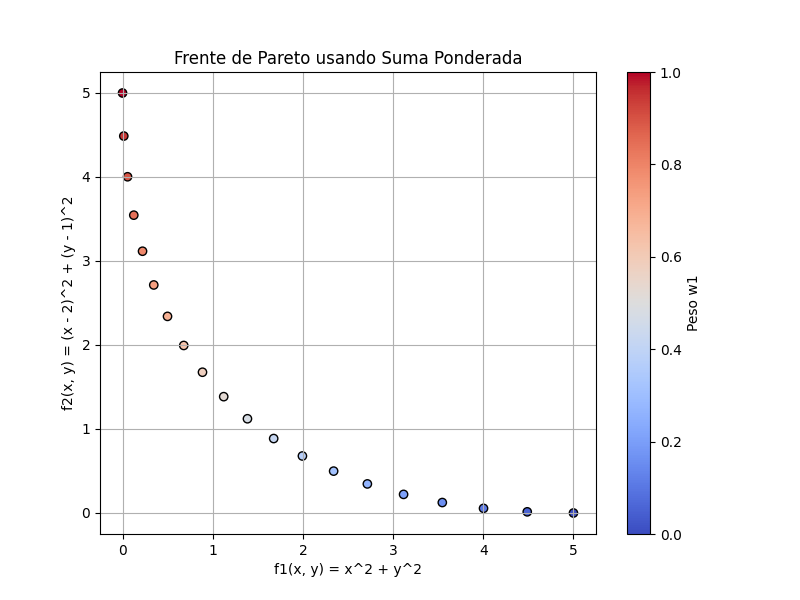
\includegraphics[width=0.9\linewidth]{Figure_3.png}
	\caption{Suma Ponderada}
	\label{fig:enter-label}
\end{figure}

Los puntos mostrados en el gráfico representan soluciones \textbf{óptimas de Pareto}, es decir, soluciones donde mejorar un objetivo implica necesariamente empeorar el otro.  

- Si \( w_1 \) es alto y \( w_2 \) es bajo, la solución se acerca al origen (minimiza \( f_1 \)).
- Si \( w_2 \) es alto y \( w_1 \) es bajo, la solución se acerca al punto \( (2,1) \) (minimiza \( f_2 \)).
- La curva en el gráfico representa el \textbf{frente de Pareto}, el conjunto de todas las soluciones óptimas dependiendo de los pesos.

El método de suma ponderada permite obtener diferentes soluciones óptimas modificando los pesos asignados a cada función objetivo. Sin embargo, este método tiene la limitación de que algunas soluciones pueden no ser alcanzables si el frente de Pareto es no convexo.


\subsubsection{Método de $\varepsilon$-Restricción}

El método de $\varepsilon$-Restricción es una técnica ampliamente utilizada en la optimización multiobjetivo para resolver problemas en los que se busca optimizar múltiples objetivos que pueden ser conflictivos entre sí. Esta metodología transforma un problema de optimización multiobjetivo en una serie de problemas de optimización de un solo objetivo, lo que facilita encontrar el conjunto de soluciones de Pareto.

El presente trabajo es un esfuerzo por implementar de manera efectiva el método $\varepsilon$-Restricción para producir las soluciones óptimas de Pareto en un MOMP. Proponemos una versión novedosa del método ($\varepsilon$–AUGMECON) que evita la producción de soluciones óptimas de Pareto débiles y acelera todo el proceso al evitar iteraciones redundantes \cite{Mavrotas2009}.

\paragraph{Definición:}
En este método, uno de los objetivos se convierte en la función objetivo principal, mientras que los demás se manejan como restricciones. Estas restricciones se imponen con un parámetro $\varepsilon$ que define el umbral máximo de tolerancia para cada uno de los otros objetivos. Al variar el valor de $\varepsilon$, se generan diferentes soluciones, que representan puntos sobre el frente de Pareto. 

El frente de Pareto, en este contexto, es el conjunto de soluciones no dominadas, es decir, aquellas soluciones que no pueden ser mejoradas en un objetivo sin empeorar otro.

\paragraph{Características del Método de $\varepsilon$-Restricción:}
\begin{itemize}
	\item \textbf{Simplicidad:} Es relativamente sencillo de implementar, ya que convierte un problema de optimización multiobjetivo en varios problemas de optimización unidimensionales.
	\item \textbf{Flexibilidad:} Permite a los tomadores de decisiones ajustar el parámetro $\varepsilon$ según las preferencias de los objetivos, explorando soluciones que equilibran los diferentes objetivos en diversos grados.
	\item \textbf{Generación de Soluciones Pareto Óptimas:} Al variar $\varepsilon$, se obtiene un conjunto de soluciones que forman el frente de Pareto, permitiendo evaluar las compensaciones entre los objetivos.
	\item \textbf{Limitaciones:} La selección adecuada de los valores de $\varepsilon$ es crucial. Valores mal definidos pueden resultar en soluciones que no representan el verdadero frente de Pareto o incluso en la imposibilidad de encontrar soluciones viables.
\end{itemize}

\paragraph{Aplicaciones del Método:}
El método de $\varepsilon$-Restricción es útil en campos como la ingeniería, la planificación urbana, la gestión de recursos naturales y la política pública. En estos campos, se utiliza para tomar decisiones informadas que involucren la optimización simultánea de varios criterios.

Como se señala en un estudio reciente, el método de $\varepsilon$-Restricción permite a los tomadores de decisiones buscar un punto de Pareto específico mediante la selección adecuada de los valores de $\varepsilon$. Esto facilita la reducción del espacio de búsqueda y mejora la eficiencia del proceso de optimización (Pirouz y Khorram, 2023).
\section*{Suma Ponderada en Optimización Multiobjetivo}
La suma ponderada es una técnica utilizada en optimización multiobjetivo para combinar varias funciones objetivo en una única función. La fórmula general es:

\[
F(x) = \sum_{i=1}^k w_i f_i(x)
\]

Donde:
\begin{itemize}
	\item \( f_i(x) \): Son las funciones objetivo individuales.
	\item \( w_i \): Son los pesos asignados a cada función objetivo (\( w_i \geq 0 \) y \( \sum_{i=1}^k w_i = 1 \)).
	\item \( x \): Es el vector de variables de decisión.
\end{itemize}

\subsection*{Diferencia con la Fórmula General}
La fórmula general de la suma ponderada:
\[
S_j = \sum_{i=1}^n w_i x_{ij}
\]
se utiliza en contextos más amplios, como el cálculo de promedios ponderados o índices compuestos. En cambio, la fórmula de la suma ponderada en optimización multiobjetivo es específica para combinar funciones objetivo en un problema de optimización.

\subsection*{Ejemplo de Aplicación}
En el ejemplo de la planificación urbana, la función objetivo combinada usando la suma ponderada es:
\[
F(x) = w_1 f_1(x) - w_2 f_2(x)
\]
donde:
\begin{itemize}
	\item \( f_1(x) \): Maximizar el acceso a servicios públicos.
	\item \( f_2(x) \): Minimizar el costo de implementación.
	\item \( w_1 \) y \( w_2 \): Pesos que representan la importancia relativa de cada objetivo.
\end{itemize}

\subsection*{Suma Ponderada y ε-Restricción}
\subsection*{Planificación Urbana}
Un gobierno local desea planificar la construcción de centros de servicios públicos en una ciudad. Los objetivos son:
\begin{itemize}
	\item \textbf{Maximizar el acceso a servicios públicos}: Cuantificado como el porcentaje de la población que vive a menos de 2 km de un centro de servicios.
	\item \textbf{Minimizar el costo de implementación}: Cuantificado como el costo total de construcción y mantenimiento de los centros.
\end{itemize}

\subsection*{Método de Suma Ponderada}
El método de suma ponderada combina los objetivos en una única función objetivo mediante la asignación de pesos:
\[
F(x) = w_1 \cdot f_1(x) + w_2 \cdot f_2(x)
\]
Donde:
\begin{itemize}
	\item \( f_1(x) \): Porcentaje de población con acceso a servicios.
	\item \( f_2(x) \): Costo total de implementación.
	\item \( w_1 \) y \( w_2 \): Pesos que representan la importancia relativa de cada objetivo (\( w_1 + w_2 = 1 \)).
\end{itemize}

\subsection*{Método de ε-Restricción}
El método de ε-restricción convierte uno de los objetivos en una restricción y optimiza el otro:
\[
\text{Maximizar } f_1(x) \quad \text{sujeto a } f_2(x) \leq \epsilon
\]

\subsection*{Ejemplo Numérico}
Supongamos los siguientes datos:
\begin{itemize}
	\item Función de acceso: \( f_1(x) = 50x \).
	\item Función de costo: \( f_2(x) = 2x \).
	\item Presupuesto máximo: 10 millones de dólares.
\end{itemize}

\subsubsection*{Aplicación del Método de Suma Ponderada}
1. Definir la función objetivo:
\[
F(x) = 0.7 \cdot (50x) - 0.3 \cdot (2x) = 34.4x
\]
2. Resolver:
\[
\text{Maximizar } 34.4x \quad \text{sujeto a } 2x \leq 10
\]
Solución: \( x = 5 \) (se construyen 5 centros).

\subsubsection*{Aplicación del Método de ε-Restricción}
1. Fijar \( \epsilon = 10 \) millones de dólares:
\[
\text{Maximizar } 50x \quad \text{sujeto a } 2x \leq 10
\]
Solución: \( x = 5 \) (se construyen 5 centros).
2. Fijar \( \epsilon = 5 \) millones de dólares:
\[
\text{Maximizar } 50x \quad \text{sujeto a } 2x \leq 5
\]
Solución: \( x = 2 \) (se construyen 2 centros).

\subsection{Algoritmos Evolutivos para Problemas Multiobjetivo}

Los algoritmos evolutivos son técnicas de optimización basadas en principios inspirados en la selección natural y la genética, que forman parte de la familia de los algoritmos de búsqueda estocástica. Estas técnicas son ampliamente utilizadas para resolver problemas complejos donde existen múltiples objetivos en conflicto. 

En el contexto de problemas multiobjetivo, los algoritmos evolutivos tienen la capacidad de generar un conjunto de soluciones que representan las mejores alternativas disponibles según las compensaciones entre diferentes objetivos. Este conjunto de soluciones conforma lo que se conoce como la \textbf{frontera de Pareto}.

La optimización multiobjetivo requiere técnicas avanzadas que permitan encontrar soluciones eficientes en problemas con múltiples objetivos en conflicto. En este contexto, los algoritmos evolutivos han demostrado ser herramientas eficaces para aproximar la frontera de Pareto. Según Coello, Lamont y Van Veldhuizen \cite{Coello2007}, estos algoritmos utilizan una población de soluciones que evolucionan mediante operadores como selección, cruza y mutación. A diferencia de los métodos tradicionales que optimizan un único objetivo, los algoritmos evolutivos generan un conjunto de soluciones que equilibran diversos objetivos en conflicto, brindando a los tomadores de decisiones un espectro de alternativas no dominadas entre sí.  

Dentro de esta línea de investigación, Sharifi et al. \cite{Sharifi2021} propusieron el algoritmo de enjambre de polillas multiobjetivo (MOMSA), una metaheurística innovadora diseñada para resolver problemas multiobjetivo de alta complejidad. Este algoritmo introduce una nueva definición de polillas exploradoras y luz de la luna, mejorando la capacidad de sincronización y asegurando una distribución equilibrada de soluciones no dominadas. Para evaluar su desempeño, MOMSA fue comparado con tres metaheurísticas ampliamente utilizadas: MOEA/D, PESA-II y MOALO. A través de métricas como la distancia generacional (GD), el espaciamiento (S), la propagación (Δ) y la propagación máxima (MS), se evidenció que MOMSA supera a estos métodos en términos de rendimiento y capacidad exploratoria, consolidándose como un modelo robusto y confiable para la optimización multiobjetivo.

\paragraph{Funcionamiento General:}
A través de un proceso evolutivo simulado, los algoritmos evolutivos iteran sobre múltiples generaciones de soluciones, mejorando gradualmente la calidad de estas. Este enfoque permite explorar grandes espacios de búsqueda, evitar quedar atrapados en óptimos locales y encontrar soluciones globales de alta calidad, incluso cuando las relaciones entre los objetivos son no lineales o complejas.

\subsubsection{Beneficios de los Algoritmos Evolutivos para Problemas Multiobjetivo}

\begin{enumerate}
	\item \textbf{Manejo de problemas complejos:} Son ideales para problemas de optimización multiobjetivo, especialmente cuando los objetivos tienen interacciones complejas o no se pueden definir de manera sencilla.
	\item \textbf{Generación de un conjunto de soluciones:} A diferencia de los enfoques tradicionales que buscan una sola solución, los algoritmos evolutivos producen un conjunto de soluciones eficientes. Esto permite a los tomadores de decisiones visualizar las compensaciones entre diferentes objetivos.
	\item \textbf{Flexibilidad y adaptabilidad:} Son adaptables a una amplia gama de problemas, con diferentes tipos de restricciones y objetivos.
	\item \textbf{Paralelización eficiente:} Estos algoritmos pueden ser paralelizados de manera efectiva, mejorando su rendimiento computacional, especialmente en problemas con muchas variables.
	\item \textbf{Evitar óptimos locales:} Gracias a su naturaleza estocástica, los algoritmos evolutivos son capaces de explorar mejor el espacio de soluciones y evitan quedar atrapados en óptimos locales.
\end{enumerate}

\subsubsection{Desventajas de los Algoritmos Evolutivos para Problemas Multiobjetivo}

\begin{enumerate}
	\item \textbf{Alto costo computacional:} Requieren numerosas evaluaciones de la función objetivo, lo que puede ser costoso, especialmente en problemas con funciones complejas.
	\item \textbf{Convergencia lenta:} La convergencia hacia una solución óptima puede ser lenta debido a la evaluación de múltiples generaciones de soluciones.
	\item \textbf{Selección de parámetros:} La elección de parámetros adecuados, como el tamaño de la población y las tasas de mutación, es crucial para el rendimiento del algoritmo.
	\item \textbf{No garantiza la solución global óptima:} Aunque los algoritmos evolutivos evitan quedar atrapados en óptimos locales, no garantizan la obtención de la mejor solución global.
	\item \textbf{Dependencia de la función objetivo:} El rendimiento puede verse afectado si las funciones objetivo son ruidosas o difíciles de evaluar.
\end{enumerate}

\section*{Ejemplo:}
Los Algoritmos Evolutivos para Problemas Multiobjetivo (MOEAs, por sus siglas en inglés) son técnicas de optimización que permiten resolver problemas con múltiples objetivos que a menudo entran en conflicto. Un ejemplo clásico es la optimización de un diseño de ingeniería donde se busca minimizar el costo y maximizar la eficiencia al mismo tiempo. En este documento, se presenta un ejemplo práctico utilizando el algoritmo NSGA-II (Non-dominated Sorting Genetic Algorithm II) implementado en Python con la biblioteca DEAP.

\section*{Bibliotecas Necesarias}
Para ejecutar el código proporcionado, se requiere instalar la biblioteca DEAP (Distributed Evolutionary Algorithms in Python). Esta biblioteca proporciona herramientas para implementar algoritmos evolutivos de manera sencilla. La instalación se puede realizar utilizando el siguiente comando:

\begin{lstlisting}[language=bash]
	pip install deap
\end{lstlisting}

\section*{Ejemplo Ssobre el algoritmo }
El siguiente ejemplo utiliza NSGA-II para resolver un problema multiobjetivo donde se busca minimizar la suma de los valores de un individuo y maximizar la suma de los cuadrados de esos valores. A continuación, se presenta el código de Python que implementa este algoritmo.

\subsection*{Código}
\begin{lstlisting}[style=python]
	import random
	from deap import base, creator, tools, algorithms
	
	# Definir los objetivos y la estructura del individuo
	creator.create("FitnessMulti", base.Fitness, weights=(-1.0, 1.0))  # Minimizar el primer objetivo, maximizar el segundo
	creator.create("Individual", list, fitness=creator.FitnessMulti)
	
	# Inicializar la caja de herramientas
	toolbox = base.Toolbox()
	
	# Definir los atributos del individuo
	toolbox.register("attr_float", random.random)
	toolbox.register("individual", tools.initRepeat, creator.Individual, toolbox.attr_float, n=10)
	toolbox.register("population", tools.initRepeat, list, toolbox.individual)
	
	# Definir la función de evaluación
	def evaluate(individual):
	obj1 = sum(individual)  # Primer objetivo: minimizar la suma de los valores
	obj2 = sum(x**2 for x in individual)  # Segundo objetivo: maximizar la suma de los cuadrados
	return obj1, obj2
	
	toolbox.register("evaluate", evaluate)
	toolbox.register("mate", tools.cxSimulatedBinaryBounded, eta=20.0, low=0, up=1)
	toolbox.register("mutate", tools.mutPolynomialBounded, eta=20.0, low=0, up=1, indpb=1.0/10)
	toolbox.register("select", tools.selNSGA2)
	
	# Configurar el algoritmo evolutivo
	def main():
	random.seed(64)
	population = toolbox.population(n=100)
	NGEN = 40
	CXPB = 0.9
	MUTPB = 0.1
	
	# Evaluar toda la población inicial
	fitnesses = list(map(toolbox.evaluate, population))
	for ind, fit in zip(population, fitnesses):
	ind.fitness.values = fit
	
	# Evolución de la población
	for gen in range(NGEN):
	offspring = algorithms.varAnd(population, toolbox, CXPB, MUTPB)
	fitnesses = list(map(toolbox.evaluate, offspring))
	for ind, fit in zip(offspring, fitnesses):
	ind.fitness.values = fit
	population = toolbox.select(population + offspring, k=len(population))
	
	# Obtener los mejores individuos
	best_individuals = tools.selBest(population, k=10)
	for bi in best_individuals:
	print(bi.fitness.values)
	
	if __name__ == "__main__":
	main()
\end{lstlisting}


\section*{Resultados de la Compilación}
Al ejecutar el código anterior, se obtienen los siguientes resultados, que representan los valores de fitness de los mejores individuos encontrados:

\begin{center}
	\begin{tabular}{|c|c|}
		\hline
		\textbf{Objetivo 1} & \textbf{Objetivo 2} \\
		\hline
		0.3407734975709522 & 0.02185017702978862 \\
		0.5204204595767217 & 0.0511122928454819 \\
		0.6346872234089597 & 0.20588259970285336 \\
		0.6917599875285423 & 0.21463212935052486 \\
		0.833715893185191 & 0.3906376301602112 \\
		0.9491136792148126 & 0.5973499224502495 \\
		0.9541358471928447 & 0.6035428485662415 \\
		1.0612164897084966 & 0.7057584475873536 \\
		1.0981698569043927 & 0.7839298333251374 \\
		1.1495297163047962 & 0.8839451258645329 \\
		\hline
	\end{tabular}
\end{center}

En este ejemplo, se ha implementado un algoritmo evolutivo multiobjetivo utilizando NSGA-II para resolver un problema donde se busca minimizar la suma de los valores de un individuo y maximizar la suma de los cuadrados de esos valores. Los resultados muestran que el algoritmo es capaz de encontrar un conjunto de soluciones que representan un equilibrio entre los dos objetivos. Este tipo de algoritmos es especialmente útil en problemas de ingeniería y diseño donde se deben considerar múltiples criterios de optimización simultáneamente. La biblioteca DEAP facilita la implementación de estos algoritmos, proporcionando una amplia gama de herramientas y operadores genéticos que pueden ser adaptados a diferentes problemas.



\subsection{Equilibrio de Compensaciones Políticas en Programas Sociales Peruanos}

Según Hayes et al. \cite{Hayes2022}, los enfoques tradicionales de aprendizaje por refuerzo y planificación basada en la teoría de decisiones suelen asumir un único objetivo o gestionar múltiples objetivos mediante una combinación lineal, lo que puede llevar a soluciones subóptimas en problemas complejos de toma de decisiones multiobjetivo. Esto es particularmente relevante en la formulación de políticas públicas, donde los responsables deben equilibrar objetivos en conflicto, como el crecimiento económico, la equidad social y la sostenibilidad ambiental. La aplicación de métodos multiobjetivo en este contexto permite diseñar estrategias más robustas, considerando un abanico de posibles soluciones y facilitando la identificación de compromisos aceptables entre actores con diferentes intereses.

Un claro ejemplo de la necesidad de enfoques multiobjetivo en la toma de decisiones políticas es el \textbf{Programa Pensión 65}, una iniciativa del gobierno peruano destinada a mejorar la calidad de vida de los adultos mayores en situación de pobreza extrema a través de una pensión mensual. La asignación de recursos en este programa debe equilibrar múltiples factores, como la cobertura geográfica, la equidad en la distribución de fondos y la sostenibilidad financiera a largo plazo. La optimización multiobjetivo puede desempeñar un papel clave en la mejora de la eficiencia del programa, permitiendo a los responsables de la toma de decisiones evaluar distintas configuraciones y priorizar soluciones que maximicen el impacto social sin comprometer la viabilidad económica.


\paragraph{Objetivo:}  
Evaluar cómo se gestionan las compensaciones entre la cobertura del programa, la distribución regional y los recursos disponibles.

\subsubsection{Datos Disponibles}
De acuerdo con los datos bimestrales del Programa Pensión 65 (2024), obtenidos de la plataforma \textit{Datos Abiertos del Gobierno de Perú} (\url{https://www.datosabiertos.gob.pe}), se dispone de las siguientes variables:

\begin{itemize}
	\item \textbf{PERIODO:} Meses en los que se registra la información de los beneficiarios.
	\item \textbf{DNI:} Identificación única del beneficiario.
	\item \textbf{PRIMER\_APELLIDO, SEGUNDO\_APELLIDO, NOMBRES:} Identificación personal de cada beneficiario.
	\item \textbf{CODIGO\_UBIGEO:} Código que indica la ubicación geográfica (departamento, provincia, distrito).
	\item \textbf{DEPARTAMENTO:} Región geográfica donde reside el beneficiario.
	\item \textbf{TIPO\_USUARIO:} Clasificación del tipo de beneficiario (por ejemplo, "regular").
	\item \textbf{LUGAR\_AGENCIA:} Lugar donde se realiza la atención o el pago.
\end{itemize}

Según los datos de la \textit{Relación Bimestral de Usuarios del Programa Pensión 65} (SEP-OCT 2024), la cantidad total de beneficiarios registrados es de 82,4351.

\subsubsection{Análisis}
Con estos datos, es posible realizar un análisis detallado del equilibrio de compensaciones en el programa \textbf{Pensión 65}. A continuación, se presentan dos áreas principales de análisis:

\begin{enumerate}
	\item \textbf{Cobertura Geográfica:}  
	Evaluar si el programa tiene una distribución equitativa de beneficiarios entre los departamentos del Perú. Esto puede lograrse calculando el número de beneficiarios por región y comparándolo con indicadores socioeconómicos, como el índice de pobreza de cada región.  
	Por ejemplo, se puede determinar cuántos beneficiarios hay en cada departamento utilizando herramientas como Excel o software estadístico (por ejemplo, con la función \texttt{COUNTIF} en Excel). Esto permitiría identificar posibles disparidades en la cobertura regional.
	
	\item \textbf{Distribución de Recursos:}  
	Analizar si las pensiones se distribuyen de manera equitativa o si existen compensaciones políticas para priorizar las zonas más necesitadas, como las áreas rurales o de difícil acceso. Este enfoque busca identificar si el gobierno asigna mayores recursos a las regiones con mayor índice de pobreza, lo que podría generar conflictos con el presupuesto disponible.
\end{enumerate}

\subsection*{Análisis del Programa Pensión 65}

El presente análisis busca evaluar la distribución de beneficiarios del programa \textbf{Pensión 65} en los distintos departamentos del Perú. Para ello, se emplea un enfoque de \textbf{optimización multiobjetivo}, considerando la cobertura y equidad en la distribución de los recursos.

\subsection*{Código}

\begin{lstlisting}[style=python]
	import pandas as pd
	import matplotlib.pyplot as plt
	import numpy as np
	
	# Cargar los datos
	datos = pd.read_csv("trama_UO_usuarios_202410.csv", encoding="latin1")
	
	# 1. Distribución de beneficiarios por departamento
	distribucion_departamento = datos["DEPARTAMENTO"].value_counts()
	print("Distribución de beneficiarios por departamento:")
	print(distribucion_departamento)
	
	# Gráfico de barras
	distribucion_departamento.plot(kind="bar", figsize=(10, 6))
	plt.title("Distribución de Beneficiarios por Departamento")
	plt.xlabel("Departamento")
	plt.ylabel("Número de Beneficiarios")
	plt.show()
	
	# 2. Porcentaje de beneficiarios por departamento
	porcentaje_beneficiarios = (distribucion_departamento / distribucion_departamento.sum()) * 100
	print("Porcentaje de beneficiarios por departamento:")
	print(porcentaje_beneficiarios)
	
	# Gráfico de pastel
	porcentaje_beneficiarios.plot(kind="pie", autopct="%1.1f%%", figsize=(8, 8))
	plt.title("Distribución de Beneficiarios por Departamento (%)")
	plt.show()
	
	# 3. Simulación de la frontera de Pareto
	coberturas = np.linspace(1000, 10000, 10)  # Rango de cobertura
	costos_simulados = coberturas * 100  # Costos proporcionales a la cobertura
	equidades_simuladas = np.random.uniform(10, 50, 10)  # Equidad aleatoria
	
	# Gráfico de la frontera de Pareto
	plt.figure(figsize=(10, 6))
	plt.scatter(coberturas, costos_simulados, c=equidades_simuladas, cmap="viridis")
	plt.colorbar(label="Equidad")
	plt.title("Frontera de Pareto: Cobertura vs Costos")
	plt.xlabel("Cobertura (Número de Beneficiarios)")
	plt.ylabel("Costos Totales")
	plt.show()
\end{lstlisting}

\subsection*{Resultados}

\begin{figure}[H]
	\centering
	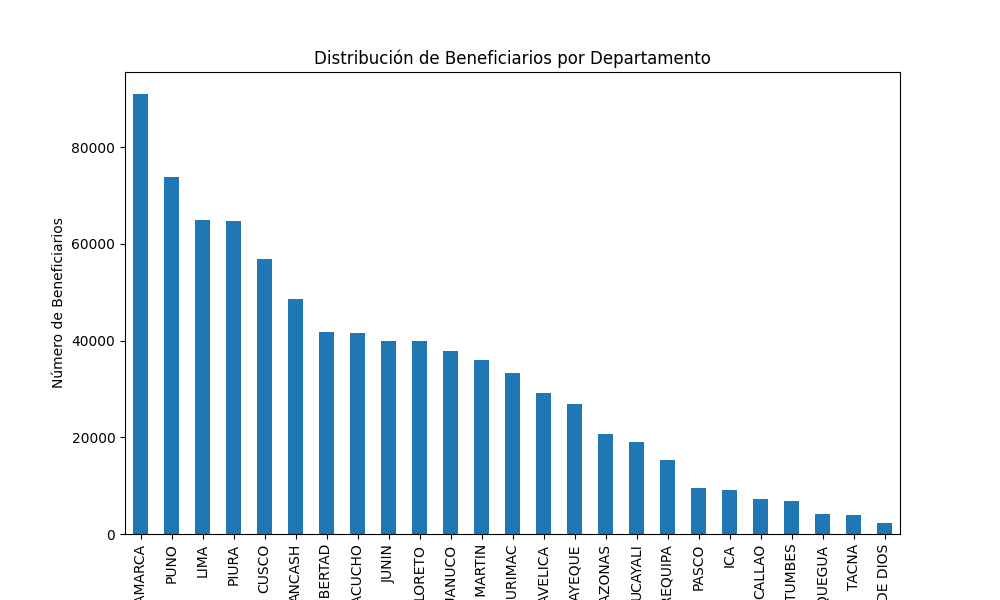
\includegraphics[width=0.9\linewidth]{Figure_1.png}
	\caption{Descripción de la imagen}
	\label{fig:mi-imagen}
\end{figure}



La ejecución del código proporciona los siguientes resultados:

\subsection*{Distribución de Beneficiarios por Departamento}

\begin{center}
	\scriptsize % Cambiar el tamaño de la fuente a más pequeño
	\begin{tabular}{|l|r|}
		\hline
		\textbf{DEPARTAMENTO} & \textbf{NÚMERO DE BENEFICIARIOS} \\
		\hline
		CAJAMARCA        & 91025                   \\
		PUNO             & 73824                   \\
		LIMA             & 65036                   \\
		PIURA            & 64772                   \\
		CUSCO            & 56794                   \\
		ANCASH           & 48540                   \\
		LA LIBERTAD      & 41764                   \\
		AYACUCHO         & 41627                   \\
		JUNIN            & 39865                   \\
		LORETO           & 39861                   \\
		HUANUCO          & 37848                   \\
		SAN MARTIN       & 35977                   \\
		APURIMAC         & 33214                   \\
		HUANCAVELICA     & 29218                   \\
		LAMBAYEQUE       & 26956                   \\
		AMAZONAS         & 20681                   \\
		UCAYALI          & 19089                   \\
		AREQUIPA         & 15404                   \\
		PASCO            & 9425                    \\
		ICA              & 9062                    \\
		CALLAO           & 7156                    \\
		TUMBES           & 6848                    \\
		MOQUEGUA         & 4036                    \\
		TACNA            & 3994                    \\
		MADRE DE DIOS    & 2335                    \\
		\hline
	\end{tabular}
\end{center}

\vspace{1cm}

\section*{Porcentaje de Beneficiarios por Departamento}

\begin{center}
	\scriptsize % Cambiar el tamaño de la fuente a más pequeño
	\begin{tabular}{|l|r|}
		\hline
		\textbf{DEPARTAMENTO} & \textbf{PORCENTAJE DE BENEFICIARIOS} \\
		\hline
		CAJAMARCA        & 10.3\%                       \\
		PUNO             & 8.4\%                        \\
		LIMA             & 7.4\%                        \\
		PIURA            & 7.3\%                        \\
		CUSCO            & 6.4\%                        \\
		ANCASH           & 5.5\%                        \\
		LA LIBERTAD      & 4.7\%                        \\
		AYACUCHO         & 4.7\%                        \\
		JUNIN            & 4.5\%                        \\
		LORETO           & 4.5\%                        \\
		HUANUCO          & 4.3\%                        \\
		SAN MARTIN       & 4.1\%                        \\
		APURIMAC         & 3.7\%                        \\
		HUANCAVELICA     & 3.3\%                        \\
		LAMBAYEQUE       & 3.0\%                        \\
		AMAZONAS         & 2.3\%                        \\
		UCAYALI          & 2.2\%                        \\
		AREQUIPA         & 1.7\%                        \\
		PASCO            & 1.1\%                        \\
		ICA              & 1.0\%                        \\
		CALLAO           & 0.8\%                        \\
		TUMBES           & 0.8\%                        \\
		MOQUEGUA         & 0.5\%                        \\
		TACNA            & 0.5\%                        \\
		MADRE DE DIOS    & 0.3\%                        \\
		\hline
	\end{tabular}
\end{center}


El análisis de la distribución de beneficiarios del Programa Pensión 65 evidencia una asignación de recursos que, en términos generales, responde a los niveles de pobreza y la cantidad de adultos mayores en situación de vulnerabilidad. Departamentos como \textbf{Cajamarca, Puno, Lima y Piura} concentran más del 30\% del total de beneficiarios, lo que refleja una alta demanda y la necesidad de asistencia social en estas regiones.  

Por otro lado, algunos departamentos como \textbf{Madre de Dios, Tacna y Moquegua} presentan una proporción considerablemente menor de beneficiarios, con menos del 1\% del total. Esta diferencia puede explicarse por una menor cantidad de adultos mayores en pobreza extrema; sin embargo, también es posible que existan barreras administrativas o dificultades en la identificación de potenciales beneficiarios que limiten su acceso al programa.  

Si bien la distribución de los recursos parece alinearse con las condiciones socioeconómicas de cada región, aún persisten desafíos en términos de \textbf{equidad y cobertura}. La subrepresentación de algunas zonas sugiere la necesidad de un análisis más detallado para garantizar que el programa llegue de manera efectiva a todas las poblaciones vulnerables. En este sentido, es fundamental continuar evaluando la eficacia del programa y explorar posibles estrategias de optimización en la asignación de recursos para mejorar su impacto social y reducir las brechas de acceso entre las distintas regiones del país.


\newpage

\begin{thebibliography}{99}
	
	\bibitem{Couckuyt2014} 
	Couckuyt, I., Deschrijver, D., \& Dhaene, T. (2014). Cálculo rápido de la probabilidad de mejora multiobjetivo y criterios de mejora esperados para la optimización de Pareto. \textit{Journal of Global Optimization, 60}, 575–594. https://doi.org/10.1007/s10898-013-0118-2
	
	\bibitem{Sengupta2016} 
	Sengupta, R. N., Gupta, A., \& Dutta, J. (Eds.). (2016). \textit{Decision Sciences: Theory and Practice} (1st ed.). CRC Press. https://doi.org/10.1201/9781315183176
	
	\bibitem{Confesor2007} 
	Confesor, R. B., Jr., \& Whittaker, G. W. (2007). Calibración automática de modelos hidrológicos con algoritmo evolutivo multiobjetivo y optimización de Pareto 1. \textit{JAWRA Journal of the American Water Resources Association}, 43(4), 981-989. 
	https://doi.org/10.1111/j.1752-1688.2007.00080.x
	
	\bibitem{Papalexopoulos2022} 
	Papalexopoulos, T. P. (2022). \textit{Multi-Objective Optimization for Public Policy} (Doctoral dissertation). Massachusetts Institute of Technology. https://hdl.handle.net/1721.1/144994
	
	\bibitem{Blank2020} 
	J. Blank y K. Deb, "Pymoo: Optimización multiobjetivo en Python", en \textit{IEEE Access}, vol. 8, pp. 89497-89509, 2020.
	https://doi.org/10.1109/ACCESS.2020.2990567
	
	\bibitem{Hayes2022} 
	Hayes, C. F., Rădulescu, R., Bargiacchi, E. et al. (2022). Una guía práctica para el aprendizaje y la planificación de refuerzo multiobjetivo. \textit{Autonomous Agents and Multi-Agent Systems}, 36, 26. https://doi.org/10.1007/s10458-022-09552-y
	
	\bibitem{Kennedy2008} 
	Kennedy, M. C., Ford, E. D., Singleton, P., Finney, M., \& Agee, J. K. (2008). Informed multi-objective decision-making in environmental management using Pareto optimality. \textit{Journal of Applied Ecology, 45}(1), 181–192. http://doi.org/10.1111/j.1365-2664.2007.01367.x
	
	\bibitem{Bradford2012} 
	Bradford, J. B., \& D'Amato, A. W. (2012). Reconocimiento de las compensaciones en la gestión de tierras con múltiples objetivos. \textit{Frontiers in Ecology and the Environment, 10}(4), 210-216. http://doi.org/10.1890/110031
	
	\bibitem{Alban2023} 
	Albán-Pérez, C. A., Serrano-Guzmán, M. F., \& Pérez-Ruiz, D. D. (2023). Weighted sums method applied for decision making in improvement towards complete street: a case study in Popayan, Colombia. \textit{Legado de Arquitectura y Diseño, 18}(34), 155-170. https://doi.org/10.36677/legado.v18i34.22130
	
	\bibitem{Marler2010}  
	Marler, R. T., \& Arora, J. S. (2010). El método de suma ponderada para la optimización multiobjetivo: nuevos conocimientos. *Structural and Multidisciplinary Optimization, 41*, 853–862. https://doi.org/10.1007/s00158-009-0460-7
	
	\bibitem{Mavrotas2009} 
	Mavrotas, G. (2009). Effective implementation of the $\varepsilon$-constraint method in Multi-Objective Mathematical Programming problems. \textit{Applied Mathematics and Computation, 213}(2), 455–465. https://doi.org/10.1016/j.amc.2009.03.037.
	
	\bibitem{Pirouz2023} 
	Pirouz, B., \& Khorram, E. (2023). A computational approach based on the $\varepsilon$-constraint method in multi-objective optimization problems. \textit{Journal of Applied Mathematics and Computation}. https://doi.org/10.17654/AS049060453
	
	\bibitem{Sharifi2021} 
	Sharifi, M. R., Akbarifard, S., Qaderi, K., et al. (2021). Un nuevo algoritmo de optimización para resolver problemas multiobjetivo. \textit{Scientific Reports, 11}, 20326. 
	https://doi.org/10.1038/s41598-021-99617-x
	
	\bibitem{Coello2007} 
	Coello, C. A., Lamont, G. B., \& Van Veldhuizen, D. A. (2007). Algoritmos Evolutivos para Problemas Multiobjetivo. En \textit{Multi-Objective Optimization: Principles and Case Studies} (pp. 1-18). Springer. https://doi.org/10.1007/978-0-387-36797-2
	
	\bibitem{MIDIS2024} 
	Ministerio de Desarrollo e Inclusión Social (MIDIS). (2024). \textit{Relación Bimestral de Usuarios del Programa Pensión 65 (periodo SEP-OCT 2024)}. Datos abiertos del Gobierno de Perú. Recuperado de https://datosabiertos.gob.pe
	
\end{thebibliography}


\end{document}
